%% ----------------------------------------------------------------
%% Thesis.tex -- MAIN FILE (the one that you compile with LaTeX)
%% ---------------------------------------------------------------- 

% Set up the document
\documentclass[a4paper, 11pt, oneside]{Thesis}  % Use the "Thesis" style, based on the ECS Thesis style by Steve Gunn
\graphicspath{Figures/}  % Location of the graphics files (set up for graphics to be in PDF format)

% Include any extra LaTeX packages required
\usepackage[square, numbers, comma, sort&compress]{natbib}  % Use the "Natbib" style for the references in the Bibliography
\usepackage{verbatim}  % Needed for the "comment" environment to make LaTeX comments
\usepackage{vector}  % Allows "\bvec{}" and "\buvec{}" for "blackboard" style bold vectors in maths
\hypersetup{urlcolor=blue, colorlinks=true}  % Colours hyperlinks in blue, but this can be distracting if there are many links.

\newcommand{\Chpref}[1]{\hyperref[#1]{Chapter~\ref*{#1}}}
\newcommand{\chpref}[1]{\hyperref[#1]{\emph{chp.}~\ref*{#1}}}
\newcommand{\Secref}[1]{\hyperref[#1]{Section~\ref*{#1}}}
\newcommand{\secref}[1]{\hyperref[#1]{\emph{sec.}~\ref*{#1}}}
\newcommand{\Apxref}[1]{\hyperref[#1]{Appendix~\ref*{#1}}}
\newcommand{\apxref}[1]{\hyperref[#1]{\emph{apx.}~\ref*{#1}}}
\newcommand{\Figref}[1]{\hyperref[#1]{Figure~\ref*{#1}}}
\newcommand{\figref}[1]{\hyperref[#1]{\emph{fig.}~\ref*{#1}}}
\newcommand{\Tblref}[1]{\hyperref[#1]{Table~\ref*{#1}}}
\newcommand{\tblref}[1]{\hyperref[#1]{\emph{tbl.}~\ref*{#1}}}
\newcommand{\Lstref}[1]{\hyperref[#1]{Listing~\ref*{#1}}}
\newcommand{\lstref}[1]{\hyperref[#1]{\emph{lst.}~\ref*{#1}}}
\newcommand{\Defref}[1]{\hyperref[#1]{Definition~\ref*{#1}}}
\newcommand{\defref}[1]{\hyperref[#1]{\emph{def.}~\ref*{#1}}}
\newcommand{\Pgeref}[1]{\hyperref[#1]{Page~\pageref*{#1}}}
\newcommand{\pgeref}[1]{\hyperref[#1]{\emph{pp.}~\pageref*{#1}}}


%% ----------------------------------------------------------------
\begin{document}
\frontmatter      % Begin Roman style (i, ii, iii, iv...) page numbering

% Set up the Title Page
\title  {Controlling Home Devices with Microsoft Kinect}
\authors  {\texorpdfstring
            {\href{your web site or email address}{Khaled Osman}}
            {Author Name}
            }
\addresses  {\groupname\\\deptname\\\univname}  % Do not change this here, instead these must be set in the "Thesis.cls" file, please look through it instead
\date       {\today}
\subject    {}
\keywords   {}

\maketitle
%% ----------------------------------------------------------------

\setstretch{1.3}  % It is better to have smaller font and larger line spacing than the other way round

% Define the page headers using the FancyHdr package and set up for one-sided printing
\fancyhead{}  % Clears all page headers and footers
\rhead{\thepage}  % Sets the right side header to show the page number
\lhead{}  % Clears the left side page header

\pagestyle{fancy}  % Finally, use the "fancy" page style to implement the FancyHdr headers

%% ----------------------------------------------------------------
% Declaration Page required for the Thesis, your institution may give you a different text to place here
\Declaration{

\addtocontents{toc}{\vspace{1em}}  % Add a gap in the Contents, for aesthetics

I, Khaled Salah, declare that this thesis titled, `Controlling Home Devices with Microsoft Kinect' and the work presented in it are my own. I confirm that:

\begin{itemize} 
\item This work was done wholly or mainly while in candidature for a research degree at this University.
 
\item Where any part of this thesis has previously been submitted for a degree or any other qualification at this University or any other institution, this has been clearly stated.
 
\item Where I have consulted the published work of others, this is always clearly attributed.
 
\item Where I have quoted from the work of others, the source is always given. With the exception of such quotations, this thesis is entirely my own work.
 
\item I have acknowledged all main sources of help.
 
\item Where the thesis is based on work done by myself jointly with others, I have made clear exactly what was done by others and what I have contributed myself.
\\
\end{itemize}
 
 
Signed:\\
\rule[1em]{25em}{0.5pt}  % This prints a line for the signature
 
Date:\\
\rule[1em]{25em}{0.5pt}  % This prints a line to write the date
}
\clearpage  % Declaration ended, now start a new page

%% ----------------------------------------------------------------
% The "Funny Quote Page"
\pagestyle{empty}  % No headers or footers for the following pages

\null\vfill
% Now comes the written in italics
\textit{``“We’re data hungry, we want it at our fingertips. At the same time, when it comes to our comfort and convenience, we want it easily and quickly with no distractions.”''}

\begin{flushright}
Geoff Godwin
\end{flushright}

\vfill\vfill\vfill\vfill\vfill\vfill\null
\clearpage  % Funny Quote page ended, start a new page
%% ----------------------------------------------------------------

% The Abstract Page
\addtotoc{Abstract}  % Add the "Abstract" page entry to the Contents
\abstract{
\addtocontents{toc}{\vspace{1em}}  % Add a gap in the Contents, for aesthetics

A thesis presented in the development of Microsoft Kinect and home automation technology by using Skeletal tracking, Voice recognition and Gesture recognition.
\ldots

}

\clearpage  % Abstract ended, start a new page
%% ----------------------------------------------------------------

\setstretch{1.3}  % Reset the line-spacing to 1.3 for body text (if it has changed)

% The Acknowledgements page, for thanking everyone
\acknowledgements{
\addtocontents{toc}{\vspace{1em}}  % Add a gap in the Contents, for aesthetics

\ldots

}
\clearpage  % End of the Acknowledgements
%% ----------------------------------------------------------------

\pagestyle{fancy}  %The page style headers have been "empty" all this time, now use the "fancy" headers as defined before to bring them back


%% ----------------------------------------------------------------
\lhead{\emph{Contents}}  % Set the left side page header to "Contents"
\tableofcontents  % Write out the Table of Contents

%% ----------------------------------------------------------------
\lhead{\emph{List of Figures}}  % Set the left side page header to "List if Figures"
\listoffigures  % Write out the List of Figures

%% ----------------------------------------------------------------
\lhead{\emph{List of Tables}}  % Set the left side page header to "List of Tables"
\listoftables  % Write out the List of Tables

%% ----------------------------------------------------------------
\setstretch{1.5}  % Set the line spacing to 1.5, this makes the following tables easier to read
\clearpage  % Start a new page
\lhead{\emph{Abbreviations}}  % Set the left side page header to "Abbreviations"
\listofsymbols{ll}  % Include a list of Abbreviations (a table of two columns)
{
% \textbf{Acronym} & \textbf{W}hat (it) \textbf{S}tands \textbf{F}or \\
\textbf{LAH} & \textbf{L}ist \textbf{A}bbreviations \textbf{H}ere \\

}

%% ----------------------------------------------------------------
\clearpage  % Start a new page
\lhead{\emph{Physical Constants}}  % Set the left side page header to "Physical Constants"
\listofconstants{lrcl}  % Include a list of Physical Constants (a four column table)
{
% Constant Name & Symbol & = & Constant Value (with units) \\
Speed of Light & $c$ & $=$ & $2.997\ 924\ 58\times10^{8}\ \mbox{ms}^{-\mbox{s}}$ (exact)\\

}

%% ----------------------------------------------------------------
\clearpage  %Start a new page
\lhead{\emph{Symbols}}  % Set the left side page header to "Symbols"
\listofnomenclature{lll}  % Include a list of Symbols (a three column table)
{
% symbol & name & unit \\
$a$ & distance & m \\
$P$ & power & W (Js$^{-1}$) \\
& & \\ % Gap to separate the Roman symbols from the Greek
$\omega$ & angular frequency & rads$^{-1}$ \\
}


%% ----------------------------------------------------------------
\mainmatter      % Begin normal, numeric (1,2,3...) page numbering
\pagestyle{fancy}  % Return the page headers back to the "fancy" style

% Include the chapters of the thesis, as separate files
% Just uncomment the lines as you write the chapters

\chapter{Introduction}

Lately, touchless interface devices have appeared in the technology world making our lives easier. Currently the average household pays over 100 dollars a month for electricity according to the U.S. Energy Information Administration. Half of those costs are to keep the motor and compressors in operation in air conditioners and heating systems. If consumers had the ability to control their home’s climate control systems remotely, they could save money without sacrificing convenience and comfort.
The idea is to extend the Kinect's potential uses from gaming to be used in different regions making more and better use of it's capabilities. This is a handicapped-friendly project that provides an easy way to control home devices using Microsoft Kinect sensor and ARDUINO board by giving certain voice commands or by doing certain gestures or even through a touchless graphical interface.


\section{Kinect Features}

The kinect sensor contains of an infrared projector, a LED light indicator, a color camera, an IR camera, a Microphone array and a tilt motor with a vertical range of -27 to 27 degrees.
The camera has an angular field of view of 57 degrees horizontally and 43 degrees vertically.
The connection between the arduino uno board and the kinect sensor is done through a USB-Serial communication.

See \Figref{fig:kinectsensor} (see \figref{fig:kinectsensor})


\begin{figure}[tbp]
  \centering
  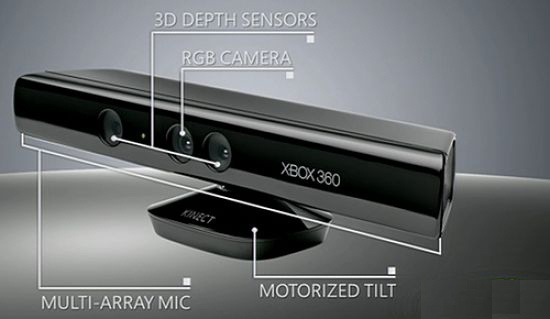
\includegraphics[width=.5\linewidth]{KinectSensor.jpg}
  \caption{Kinect sensor}
  \label{fig:kinectsensor}
\end{figure}
  
\begin{figure}[tp]
  \centering
  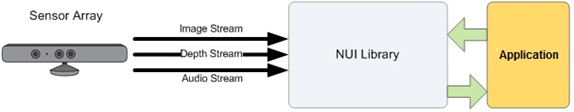
\includegraphics[width=1.0\linewidth]{KinectDataStream.png}
  \caption{Data stream}
  \label{fig:datastream}
\end{figure}
  

\subsection{Skeletal Tracking}

The Microsoft SDK provides the player's skeleton as an array of joints of a Vector4 value each, which contains each joint's x,y,z and w values; it's x,y,z position values in 3d space and the w value that indicates  the quality level (Range between 0-1)) of the position that indicates the center of mass for that skeleton which is only 1 for passive fully tracked players. The kinect sensor can detect up to 6 players at the same time, however it can only track 2 at the same time while it only stores some basic information like position values for the other 4.
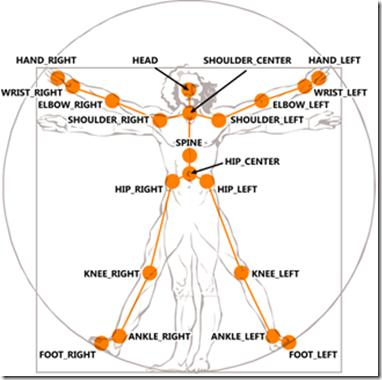
\includegraphics[scale=2]{SkeletonJoints.png}

\subsection{Speech Recognition}

The microphone array of the kinect sensor is responsible for it's hearing, by integrating it's features and creating grammars the kinect can be used for voice recognition.

\subsection{Gesture Recognition}

There's many ways you could build a gesture recognition system using the kinect SDK for example you can store your gestures as frame images and use image proccessing to compare them, or you can just compare the angle between certain joints but this won't be as efficient as it may detect other random gestures too, so it's better to compare joint positions relatively to eachothers or draw imagionary vectors between the joints and compare them to the expected directions. 
You can divide the gesture into smaller gesture parts/segments if needed and check if they succeed in each frame according to their topological order in a certain number of frames then the gesture succeeds.
In this project, the gesture recognition system does all of the above except image proccessing as there was no gesture recording software compatible with the microsoft sdk found.

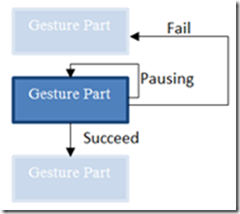
\includegraphics[width=1.0\linewidth]{GestureArchitecture1.png}
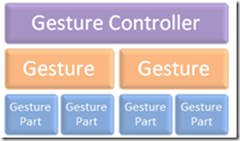
\includegraphics[width=1.0\linewidth]{GestureArchitecture2.png}

\section{Arduino}

The Arduino Uno is a microcontroller board based on the ATmega328 . It has 14 digital input/output pins of which 6 can be used as PWM outputs, 6 analog inputs, a 16 MHz ceramic resonator, a USB connection, a power jack, an ICSP header, and a reset button.
The power pins are as follows:
The ATmega328 has a 32 KB memory (with 0.5 KB used for the bootloader). It also has 2 KB of SRAM and 1 KB of EEPROM.
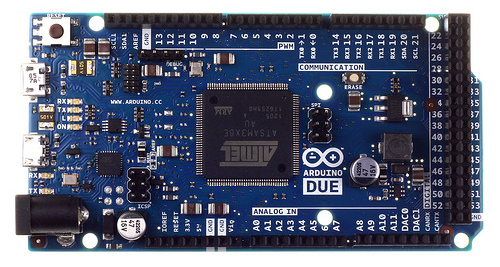
\includegraphics[scale=2]{ArduinoUNOBoard.jpg}

\subsection{Kinect-Arduino-HomeDevice physical Connection}

The connection between the kinect and the arduino is handled through a USB to Serial converter and an interface handling the websockets.
The connection between the arduino and the home devices is made through an electric circuit using sensors, relays, transistors, resistors, LEDS and an LCD etc..
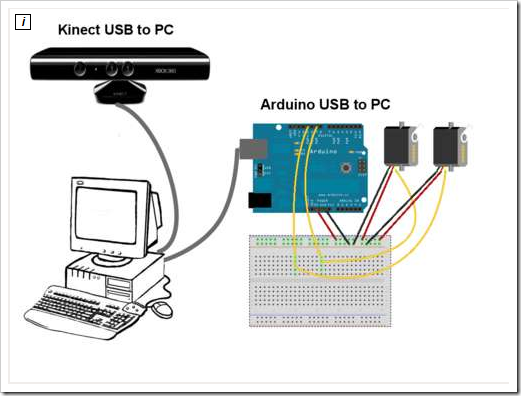
\includegraphics[scale=2]{Kinect-Arduino-Connection.png}

\section{User Stories}

The user stories and the program features are as follows:
\begin{itemize}
\item As a user, I can turn the lights on/off by entering/leaving the room.
\item As a system, I should be able to recognize certain gestures and control the device accordingly.
\item As a user, I can interact with a touchless interface.
\item As a system, I should recognize the user's face and keep track of it.
\item As a user, I can give certain voice commands.
\item As a system, I should have a circuit connection between the arduino board and the device I want to control.
\item As a system, I should be able to control the device and switch it on/off when needed.
\item As a system, I should create an interface to allow the communication between the kinect sensor and arduino board.
\item As  a user, I should see pop-up screens to show feedback from the interface at certain circumstances.
\item As a user, I should see an avatar which represents my distance to the kinect.
\item As a user, I should see an introductory fading screen to the application.
\item As a user, I can play music.
\item As a user, I should see a main screen where I can edit settings and enable/disable features like face/depth/voice/skeletal tracking.
\item As a user, I should see a screen for each controlled device where I can edit it's settings manually.
\item As a system I should provide a way for the user to enter a password to be able to manage the application.
\end{itemize}

\section{Software Architecture}

The software architecture of the project is shown in the figures below
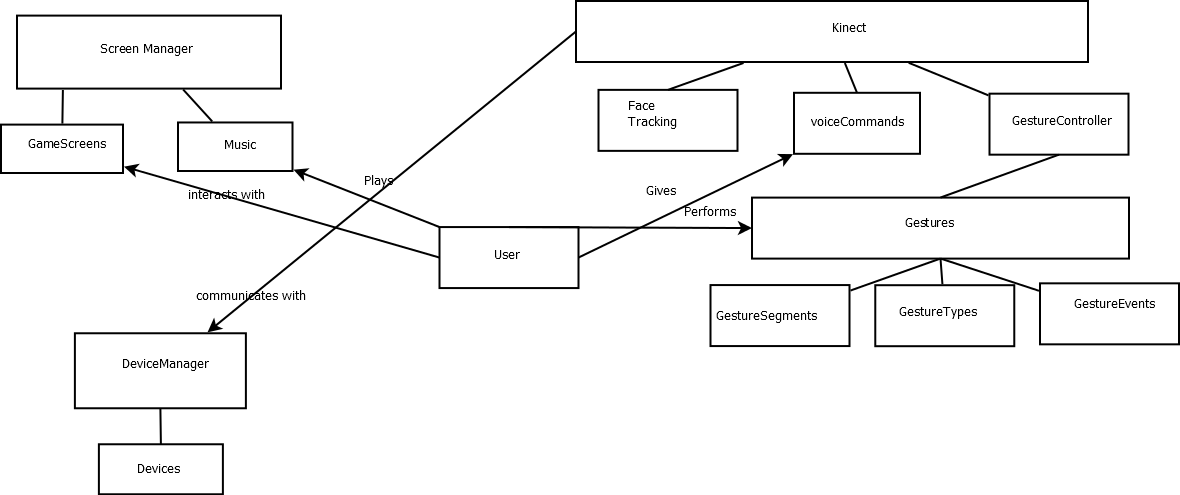
\includegraphics[width=0.8\linewidth]{SoftwareArchitecture}

%%% Local Variables: 
%%% mode: latex
%%% TeX-master: "../Thesis"
%%% End: 
 % Introduction

%\input{Chapters/Chapter2} % Background Theory 

%\input{Chapters/Chapter3} % Experimental Setup

%\input{Chapters/Chapter4} % Experiment 1

%\input{Chapters/Chapter5} % Experiment 2

%\input{Chapters/Chapter6} % Results and Discussion

%\input{Chapters/Chapter7} % Conclusion

%% ----------------------------------------------------------------
% Now begin the Appendices, including them as separate files

\addtocontents{toc}{\vspace{2em}} % Add a gap in the Contents, for aesthetics

\appendix % Cue to tell LaTeX that the following 'chapters' are Appendices

\chapter{An Appendix}

http://msdn.microsoft.com/en-us/library/jj131025.aspx
http://arduino.cc/en/Main/arduinoBoardUno
http://blogs.msdn.com/b/mcsuksoldev/archive/2011/08/08/writing-a-gesture-service-with-the-kinect-for-windows-sdk.aspx
Beginning kinect programming with the microsoft kinect sdk book
Arduino cookbook


%Lorem ipsum dolor sit amet, consectetur adipiscing elit. Vivamus at pulvinar nisi. Phasellus hendrerit, diam placerat interdum iaculis, mauris justo cursus risus, in viverra purus eros at ligula. Ut metus justo, consequat a tristique posuere, laoreet nec nibh. Etiam et scelerisque mauris. Phasellus vel massa magna. Ut non neque id tortor pharetra bibendum vitae sit amet nisi. Duis nec quam quam, sed euismod justo. Pellentesque eu tellus vitae ante tempus malesuada. Nunc accumsan, quam in congue consequat, lectus lectus dapibus erat, id aliquet urna neque at massa. Nulla facilisi. Morbi ullamcorper eleifend posuere. Donec libero leo, faucibus nec bibendum at, mattis et urna. Proin consectetur, nunc ut imperdiet lobortis, magna neque tincidunt lectus, id iaculis nisi justo id nibh. Pellentesque vel sem in erat vulputate faucibus molestie ut lorem.

%Quisque tristique urna in lorem laoreet at laoreet quam congue. Donec dolor turpis, blandit non imperdiet aliquet, blandit et felis. In lorem nisi, pretium sit amet vestibulum sed, tempus et sem. Proin non ante turpis. Nulla imperdiet fringilla convallis. Vivamus vel bibendum nisl. Pellentesque justo lectus, molestie vel luctus sed, lobortis in libero. Nulla facilisi. Aliquam erat volutpat. Suspendisse vitae nunc nunc. Sed aliquet est suscipit sapien rhoncus non adipiscing nibh consequat. Aliquam metus urna, faucibus eu vulputate non, luctus eu justo.

%Donec urna leo, vulputate vitae porta eu, vehicula blandit libero. Phasellus eget massa et leo condimentum mollis. Nullam molestie, justo at pellentesque vulputate, sapien velit ornare diam, nec gravida lacus augue non diam. Integer mattis lacus id libero ultrices sit amet mollis neque molestie. Integer ut leo eget mi volutpat congue. Vivamus sodales, turpis id venenatis placerat, tellus purus adipiscing magna, eu aliquam nibh dolor id nibh. Pellentesque habitant morbi tristique senectus et netus et malesuada fames ac turpis egestas. Sed cursus convallis quam nec vehicula. Sed vulputate neque eget odio fringilla ac sodales urna feugiat.

%Phasellus nisi quam, volutpat non ullamcorper eget, congue fringilla leo. Cras et erat et nibh placerat commodo id ornare est. Nulla facilisi. Aenean pulvinar scelerisque eros eget interdum. Nunc pulvinar magna ut felis varius in hendrerit dolor accumsan. Nunc pellentesque magna quis magna bibendum non laoreet erat tincidunt. Nulla facilisi.

%Duis eget massa sem, gravida interdum ipsum. Nulla nunc nisl, hendrerit sit amet commodo vel, varius id tellus. Lorem ipsum dolor sit amet, consectetur adipiscing elit. Nunc ac dolor est. Suspendisse ultrices tincidunt metus eget accumsan. Nullam facilisis, justo vitae convallis sollicitudin, eros augue malesuada metus, nec sagittis diam nibh ut sapien. Duis blandit lectus vitae lorem aliquam nec euismod nisi volutpat. Vestibulum ornare dictum tortor, at faucibus justo tempor non. Nulla facilisi. Cras non massa nunc, eget euismod purus. Nunc metus ipsum, euismod a consectetur vel, hendrerit nec nunc.	% Appendix Title

%\input{Appendices/AppendixB} % Appendix Title

%\input{Appendices/AppendixC} % Appendix Title

\addtocontents{toc}{\vspace{2em}}  % Add a gap in the Contents, for aesthetics
\backmatter

%% ----------------------------------------------------------------
\label{Bibliography}
\lhead{\emph{Bibliography}}  % Change the left side page header to "Bibliography"
\bibliographystyle{unsrtnat}  % Use the "unsrtnat" BibTeX style for formatting the Bibliography
\bibliography{Bibliography}  % The references (bibliography) information are stored in the file named "Bibliography.bib"

\end{document}  % The End
%% ----------------------------------------------------------------
